\documentclass[11pt]{article}
\usepackage[paperwidth=30cm,paperheight=30cm,margin=5mm]{geometry}
\usepackage[T1]{fontenc}
\usepackage{tikz}
\usetikzlibrary{arrows.meta,positioning,fit,backgrounds,calc,shapes.geometric}
\pagestyle{empty}
\tikzset{
  box/.style={draw, rounded corners=2pt, align=center, font=\small, minimum height=9mm, inner sep=4pt, fill=white},
  data/.style={box, fill=blue!8},
  model/.style={box, fill=orange!12},
  outp/.style={box, fill=green!10},
  frozen/.style={box, dashed, font=\small\itshape},
  arr/.style={-{Latex[length=2mm]}, semithick},
  lbl/.style={font=\scriptsize, align=center},
  group/.style={draw, rounded corners=4pt, dashed, gray, inner sep=6pt},
  glbl/.style={font=\scriptsize\itshape, gray, anchor=south west, inner sep=1pt}}
\begin{document}

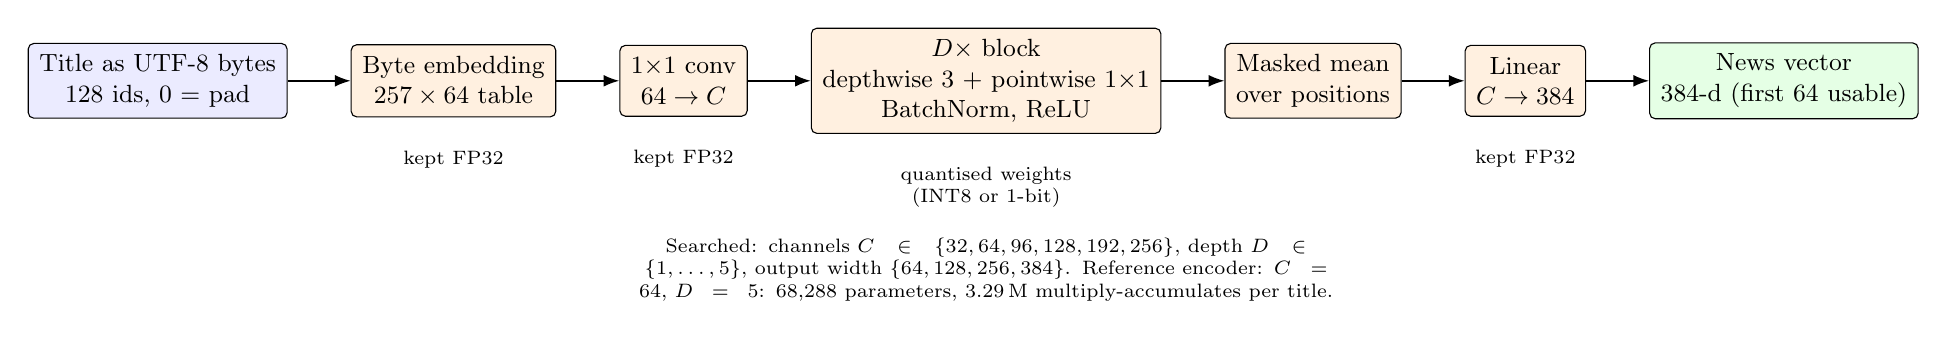
\begin{tikzpicture}[node distance=5mm and 8mm, every node/.style={font=\small}]
  \node[data] (in) {Title as UTF-8 bytes\\$128$ ids, 0 = pad};
  \node[model, right=of in] (emb) {Byte embedding\\$257 \times 64$ table};
  \node[model, right=of emb] (proj) {$1{\times}1$ conv\\$64 \to C$};
  \node[model, right=of proj] (blk) {$D \times$ block\\depthwise $3$ + pointwise $1{\times}1$\\BatchNorm, ReLU};
  \node[model, right=of blk] (pool) {Masked mean\\over positions};
  \node[model, right=of pool] (head) {Linear\\$C \to 384$};
  \node[outp, right=of head] (vec) {News vector\\384-d (first 64 usable)};
  \draw[arr] (in) -- (emb); \draw[arr] (emb) -- (proj); \draw[arr] (proj) -- (blk);
  \draw[arr] (blk) -- (pool); \draw[arr] (pool) -- (head); \draw[arr] (head) -- (vec);
  \node[lbl, below=3mm of emb] {kept FP32};
  \node[lbl, below=3mm of proj] {kept FP32};
  \node[lbl, below=3mm of blk] {quantised weights\\(INT8 or 1-bit)};
  \node[lbl, below=3mm of head] {kept FP32};
  \node[lbl, below=12mm of blk, text width=11cm] {Searched: channels $C \in \{32, 64, 96, 128, 192, 256\}$, depth $D \in \{1,\dots,5\}$, output width $\{64, 128, 256, 384\}$. Reference encoder: $C=64$, $D=5$: 68,288 parameters, 3.29\,M multiply-accumulates per title.};
\end{tikzpicture}
\end{document}
